% You should title the file with a .tex extension (hw1.tex, for example)
\documentclass[a4paper, 11pt]{article}

\usepackage{amsmath}
\usepackage{amssymb}
\usepackage{fancyhdr}
\usepackage{graphicx}

\usepackage[margin=1in]{geometry}

\newcommand{\question}[2] {\vspace{.25in} \hrule\vspace{0.5em}
\noindent{\bf #1: #2} \vspace{0.5em}
\hrule \vspace{.10in}}
\renewcommand{\part}[1] {\vspace{.10in} {\bf (#1)}}

\newcommand{\myname}{Natthakan Euaumpon}
\newcommand{\myemail}{natthakaneuaumpon@gmail.com}
\newcommand{\myhwnum}{1}

\setlength{\parindent}{0pt}
\setlength{\parskip}{5pt plus 1pt}
 
\pagestyle{fancyplain}
\lhead{\fancyplain{}{\textbf{HW\myhwnum}}}      % Note the different brackets!
\rhead{\fancyplain{}{\myname\\ \myemail}}
\chead{\fancyplain{}{ICCS310 }}

\begin{document}

\medskip                        % Skip a "medium" amount of space
                                % (latex determines what medium is)
                                % Also try: \bigskip, \littleskip

\thispagestyle{plain}
\begin{center}                  % Center the following lines
{\Large ICCS310: Assignment \myhwnum} \\
\myname \\
\myemail \\
January 2021 \\
\end{center}

\question{1}{Review: Something about Sets}
\part{1}\\
First we need to prove that  $\overline{A_1 \cup A_2 \cup A_3} \subseteq \overline{A_1} \cap \overline{A_2} \cap \overline{A_3}$.\\
To show $\overline{A_1 \cup A_2 \cup A_3} \subseteq \overline{A_1} \cap \overline{A_2} \cap \overline{A_3}$. Let $x \in \overline{A_1 \cup A_2 \cup A_3}$ according to the definition of complement if $x \in \overline{A_1 \cup A_2 \cup A_3}$ then $x \notin A_1 \cup A_2 \cup A_3$. Since they are union with each other we know that $x \notin A_1, x \notin A_2$ and $\notin A_3$. So $x \in \overline{A_1}, x \in \overline{A_2}$ and $x \in \overline{A_3}$. Therefore $x \in \overline{A_1} \cap \overline{A_2} \cap \overline{A_3}$.\\

\part{2}\\
First we need to prove that $\overline{A_1 \cap A_2} \subseteq \overline{A_1} \cup \overline{A_2}$.\\
To show that, let $x \in \overline{A_1 \cap A_2}$. We get $x \notin A \cap B$ according to the definition of compliment. So $x \notin A$ or $x \notin B$. This means $x \in \overline{A_1}$ or $x \in \overline{A_2}$. Therefore $x \in \overline{A_1} \cup \overline{A_2}$.

\question{2}{Prime and Irrational}
\part{1}\\
Let $a = p_{1} \cdot p_{2} \cdot p_{3} \cdot ... \cdot p_{n}$. Where $p_{1}, p_{2},..., p_{n} \geq 2$ and $a$ is a positive integer. Therefore $a^2 = p_{1}^2 \cdot p_{2}^2 \cdot ... \cdot p_{n}^2$. If $p$ divides $a^{2}$ this means the prime factors for $a^2$ are $p_1, p_2, ... p_n$. So $p$ is one of $p_1, p_2,..., p_n$, as $a = p_{1} \cdot p_{2} \cdot p_{3} \cdot ... \cdot p_{n}$ we can concluded that p divides a.

\part{2}\\
Let assume for the sake of contradiction. Let $\sqrt{p}$ be a rational number. This means $\sqrt{p} = \frac{a}{b}$. Where $a,b \in \mathbb{Z}, b \neq 0$ and $\frac{a}{b}$ is in least fraction. By squaring both side we get $p = \frac{a^2}{b^2}$, $b^2 = \frac{a^2}{p}$. From this we know that $p$ divides $a^2$ and according to the first part of question 2 we know that $p$ divides $a$. Let $a = p \cdot q$ where $q \in \mathbb{Z}$. So we get $b^2 = \frac{(pq)^2}{p} = \frac{p^2 \cdot q^2}{p} = p \cdot q^2$. Divide both side by p we get $q^2 = \frac{b^2}{p}$. This contradict because $\frac{a}{b}$ is in least fraction. This means $a$ and $b$ has no common factor. Therefore $\sqrt{p}$ is irrational.

\question{3}{Spacing}
Let S be a set of n+1 integer. Theres n possible way to get a pair of consecutive numbers. Let elements in set be pigeon and n possible ways to get consecutive pair be holes. According to the pigeon holes principle, since there are greater nuber of pigeons than the number of holes so there should be at least one hole with 2 or more pigeons. Therefore this guarantee that there is at least a pair $a,b \in S$ such that $a$ and $b$ are consecutive number.

\question{4}{Curious fact about graph}
Let n be the total nodes of graph $G = (V,E)$.\\
There are 2 cases, one where every node are connected with each other and one where there's node with 0 degrees.\\
First case:\\
If all the nodes are connected then the maximum number of degree a node can have is $n-1$ and the minimum is one. So you have $n-1$. You have n nodes and n-1 available degrees. So let total number of nodes be pideons and $n-1$ possible degrees then according to the pigeon hole principle, there should be 2 nodes with equal degree.\\
Second case:\\
 If a degrees 0 exist then the total nodes that connect to each other decreases. Then the total number of nodes that are connected with each other become $n-1$. So the max number of degrees a node can have is n-2 and the minimum is 0. So let total number of nodes be pideons and $n-1$ possible degrees then according to the pigeon hole principle, there should be 2 nodes with equal degree.\\
 
 \question{5}{Basic DFAs}
 \part{1}\\
 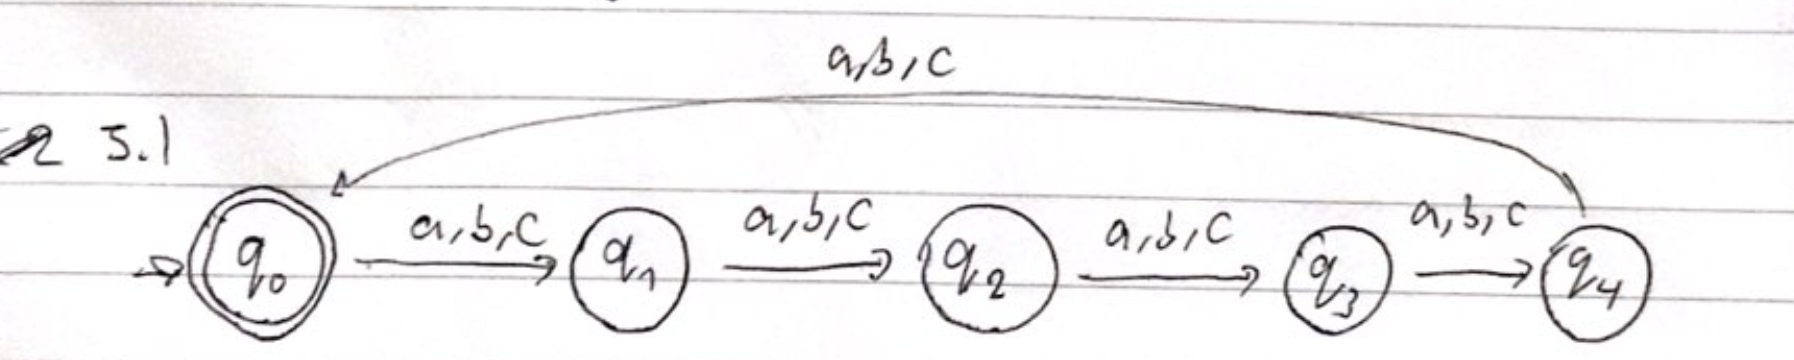
\includegraphics[width=\textwidth]{Q5-1.png}\\
 \begin{enumerate}
 	\item $q_0$ - accepting state. We want the length that is divisible by 5. So starting from $q_0$ it accpet every string that length is divisible by 5. Coming back to $q_0$ is the same as recount so every time it come back to $q_0 means string is divisible by 5$.
 	\item $q_1,q_2,q_3,q_4$ - works as a counter from 1 to 4.  When the length is 5 it goes back to $q_0$. Then the counter is reset and start comting again at $q_1$. 
 \end{enumerate}

\part{2}\\
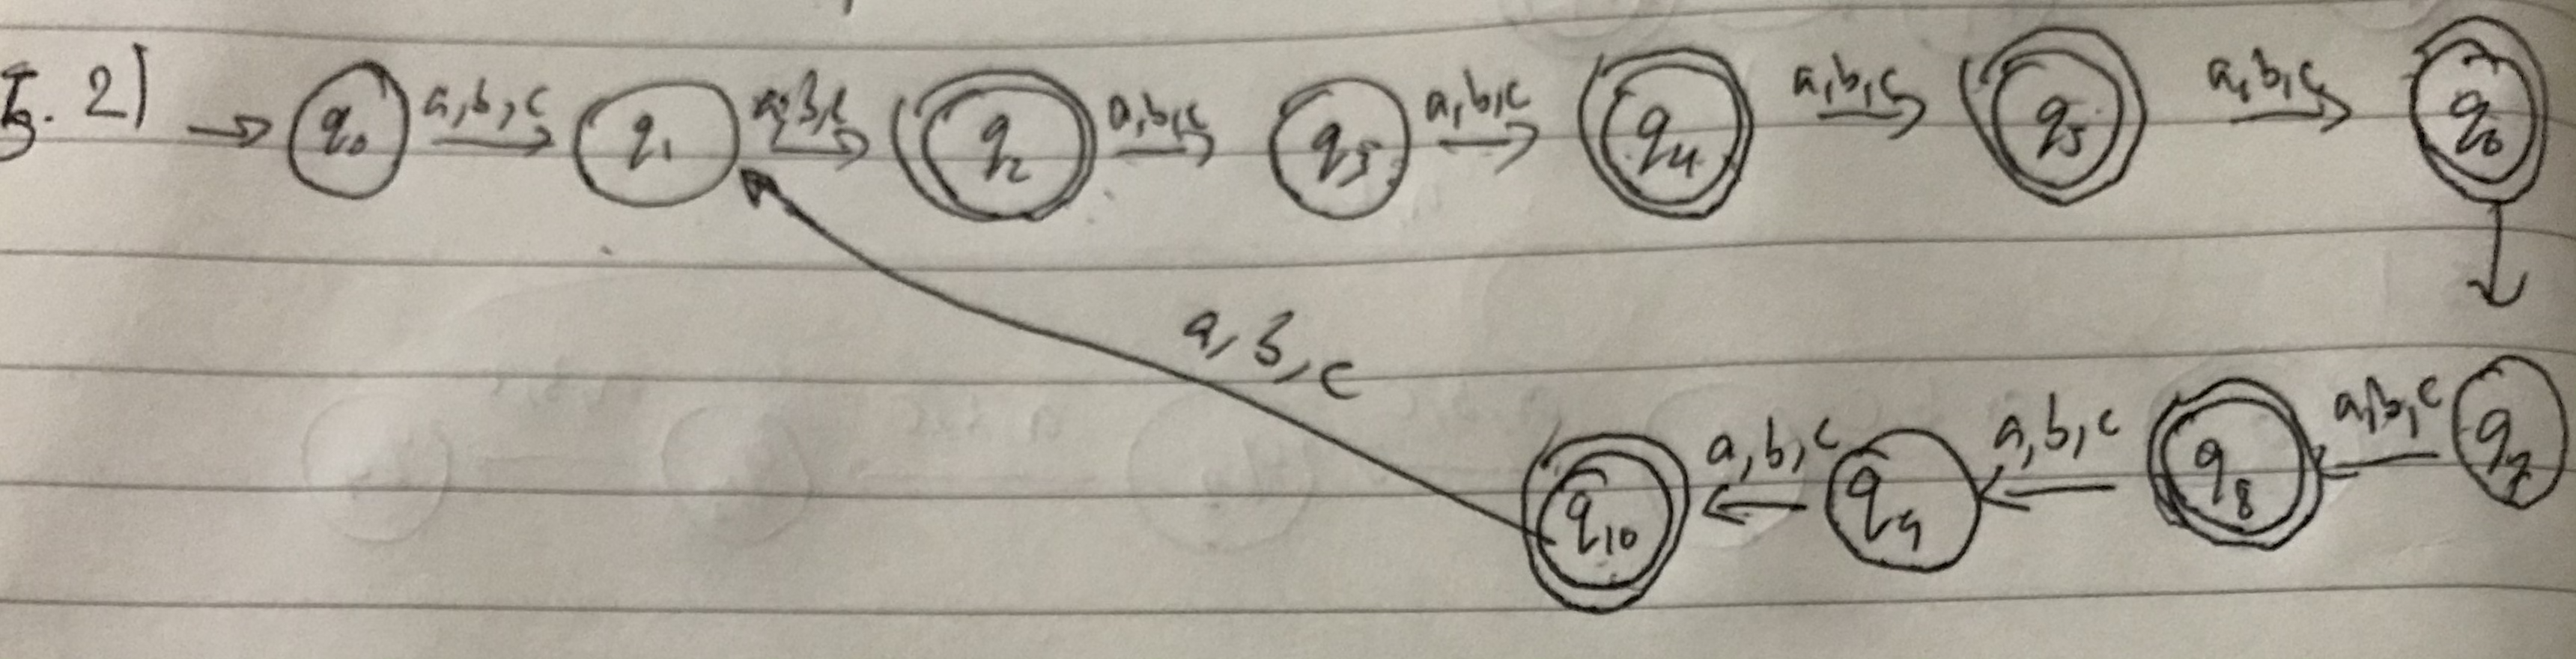
\includegraphics[width=\textwidth]{Q5-2.png}\\
Every state except accepting state works as a counter from 1 to 10.\\
\begin{enumerate}
	\item $q_0$ - starting state.
	\item $q_2, q_4, q_6, q_8$ - even length counter. Accepting state as the lenght is even.
	\item $q_5,q_10$ - Number that is divisible by five can be both even and odd. So we need 2 accepting state for both even and odd.
\end{enumerate}

\part{3}\\
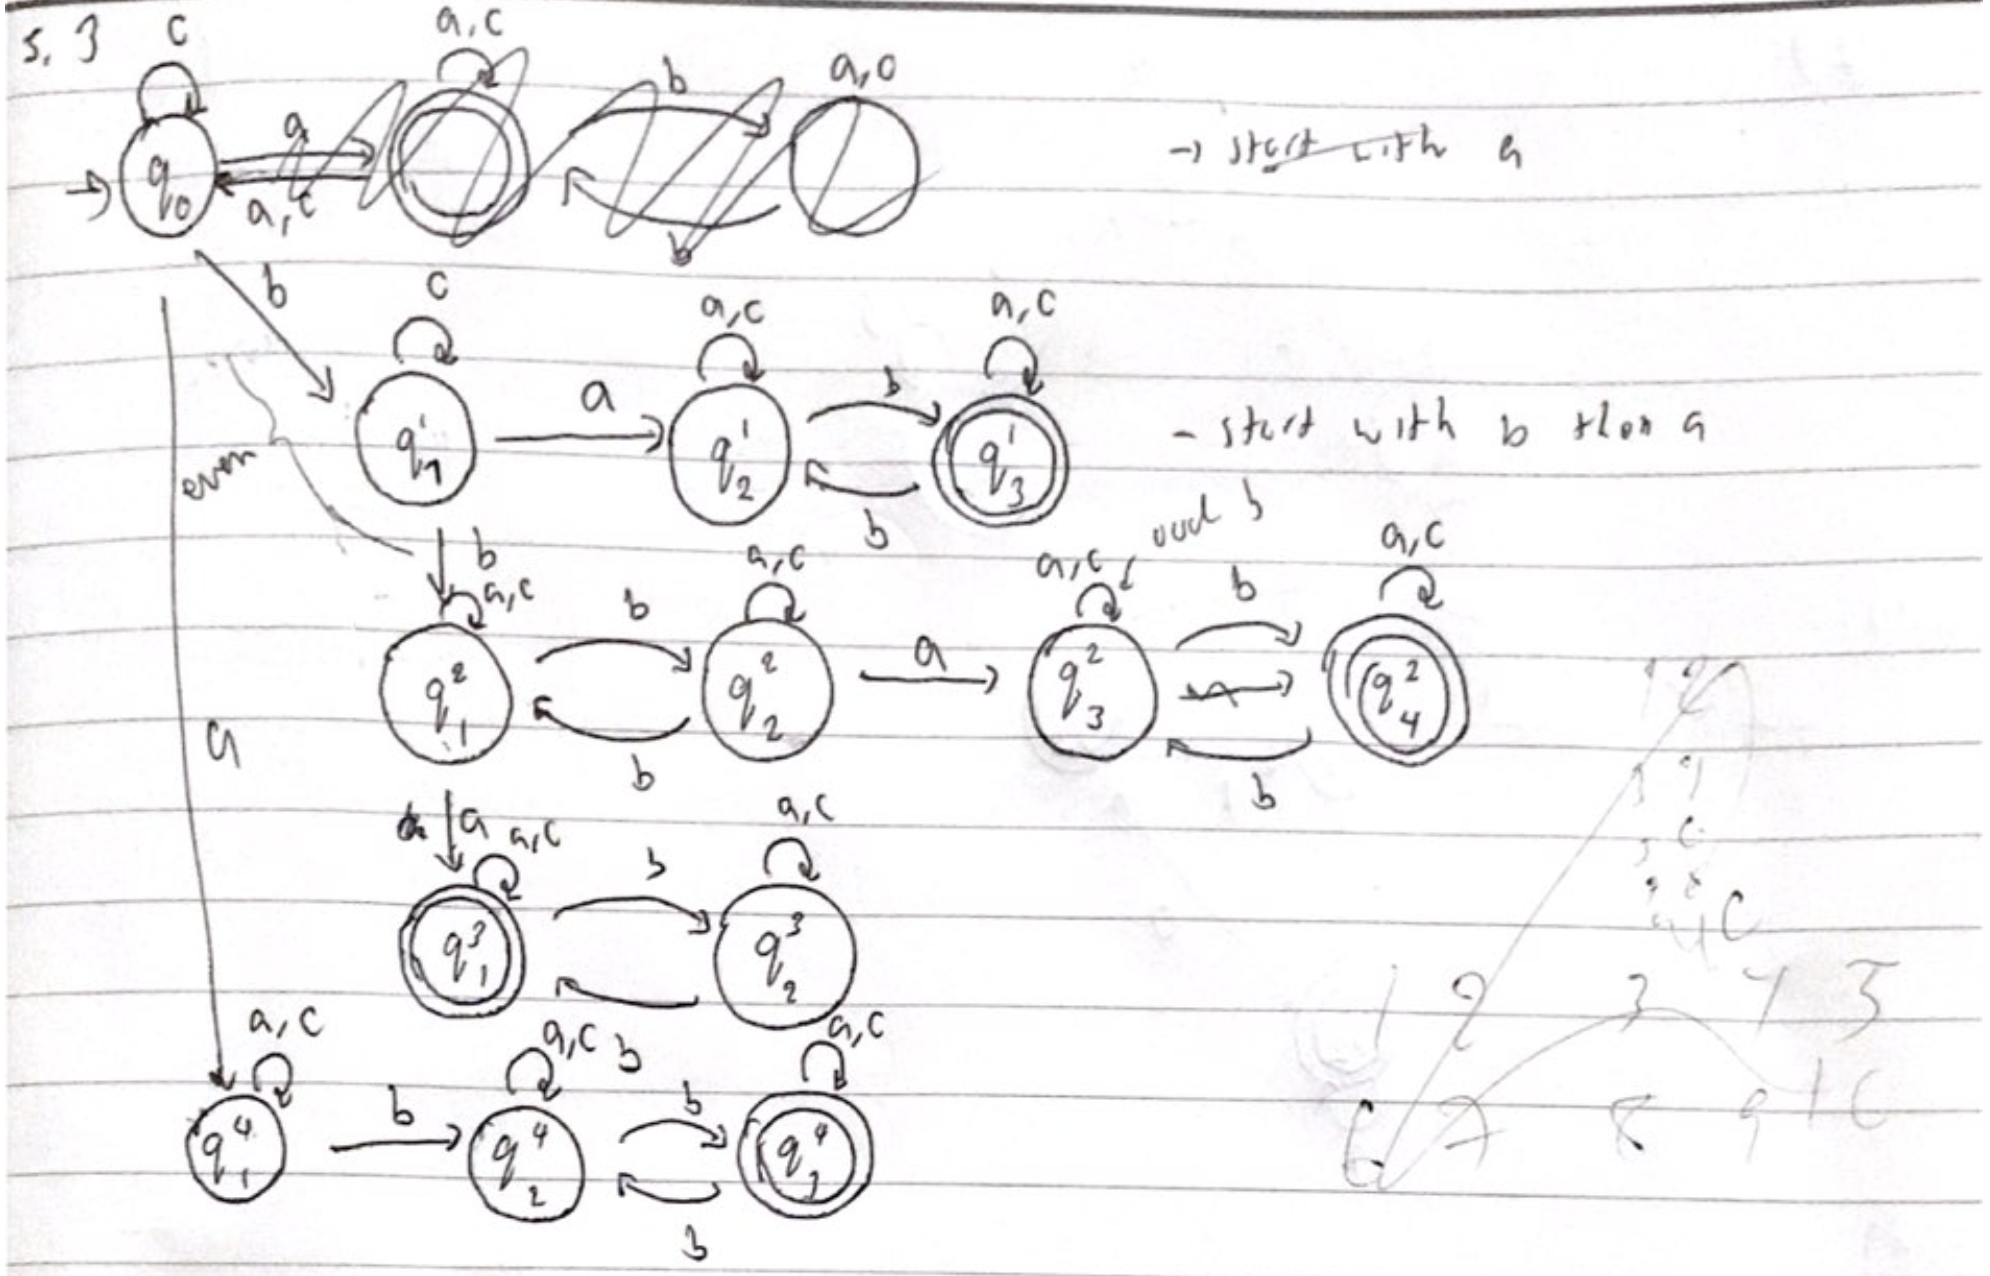
\includegraphics[width=\textwidth]{Q5-3.png}\\
\begin{enumerate}
	\item $q_0^1$ - if the first character is c do nothing because we don't need it. If it is a then we only need to only check if b is even or not. If the first character is b then we need odd number of bs and an a.
	\item $q_1^1$ - if we got c stay the smae if we get a then go to $q_2^1$ else go to $q_1^2$.
	\item $q_2^1,q_3^1$ - we already have a b so we  need odd number of bs. For getting into $q_2^1$ means we already have 1 bs and an a. So we need to check if we have odd number of bs. If it is odd then combine with the first b we will get even number of b.
	\item $q_1^2, q_2^2$ -We have even number of b and no a's. S we continue to find for a. If b is odd then a it will go to $q_3^2$. Else if b is even then it will go to $q_1^3$.
	\item $q_3^2, q_4^2$ - we already have odd bs and a. This 2 state is an odd counter for b. As we alredy odd number for b.
	\item $q_1^3, q_2^3$ - We already have even numbers of b and an a. So, we need to only make sure that the others upcoming b is even.
	\item $q_2^4, q_3^4$ - We already have and a so we need to count to make sure that b is even. 
\end{enumerate}
 
 \question{6}{Penultimate}
 \part{1}\\
 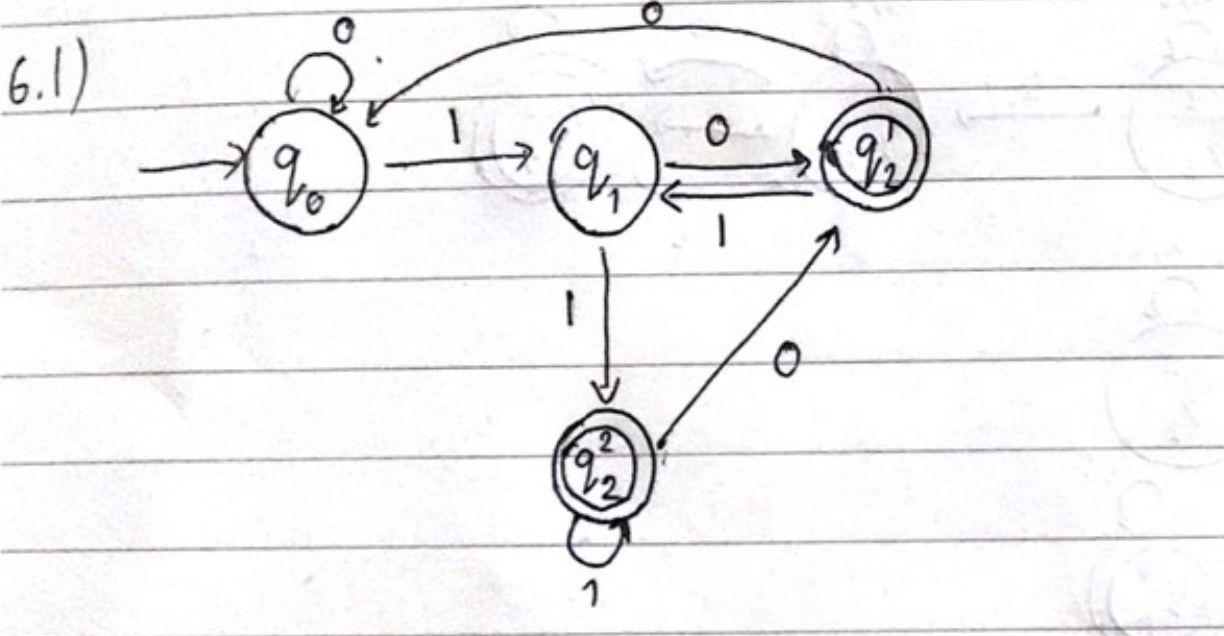
\includegraphics[width=\textwidth]{Q6-1.png}\\
 \begin{enumerate}
 	\item $q_0$ - starting state. If the first character is 0 then it will loop to itself.
 	\item $q_1$ to $q_2^1$ - we already have one if next is character and last character is 0 then it accept. if it is 1 go back to $q_1$.
 	\item $q_1$ to $q_2^2$ - if the next character is one then will continue to loop as it guarantee that second to last character is one. Else it will go to $q_2^1$
 \end{enumerate}

\question{7}{Digit Sum}
 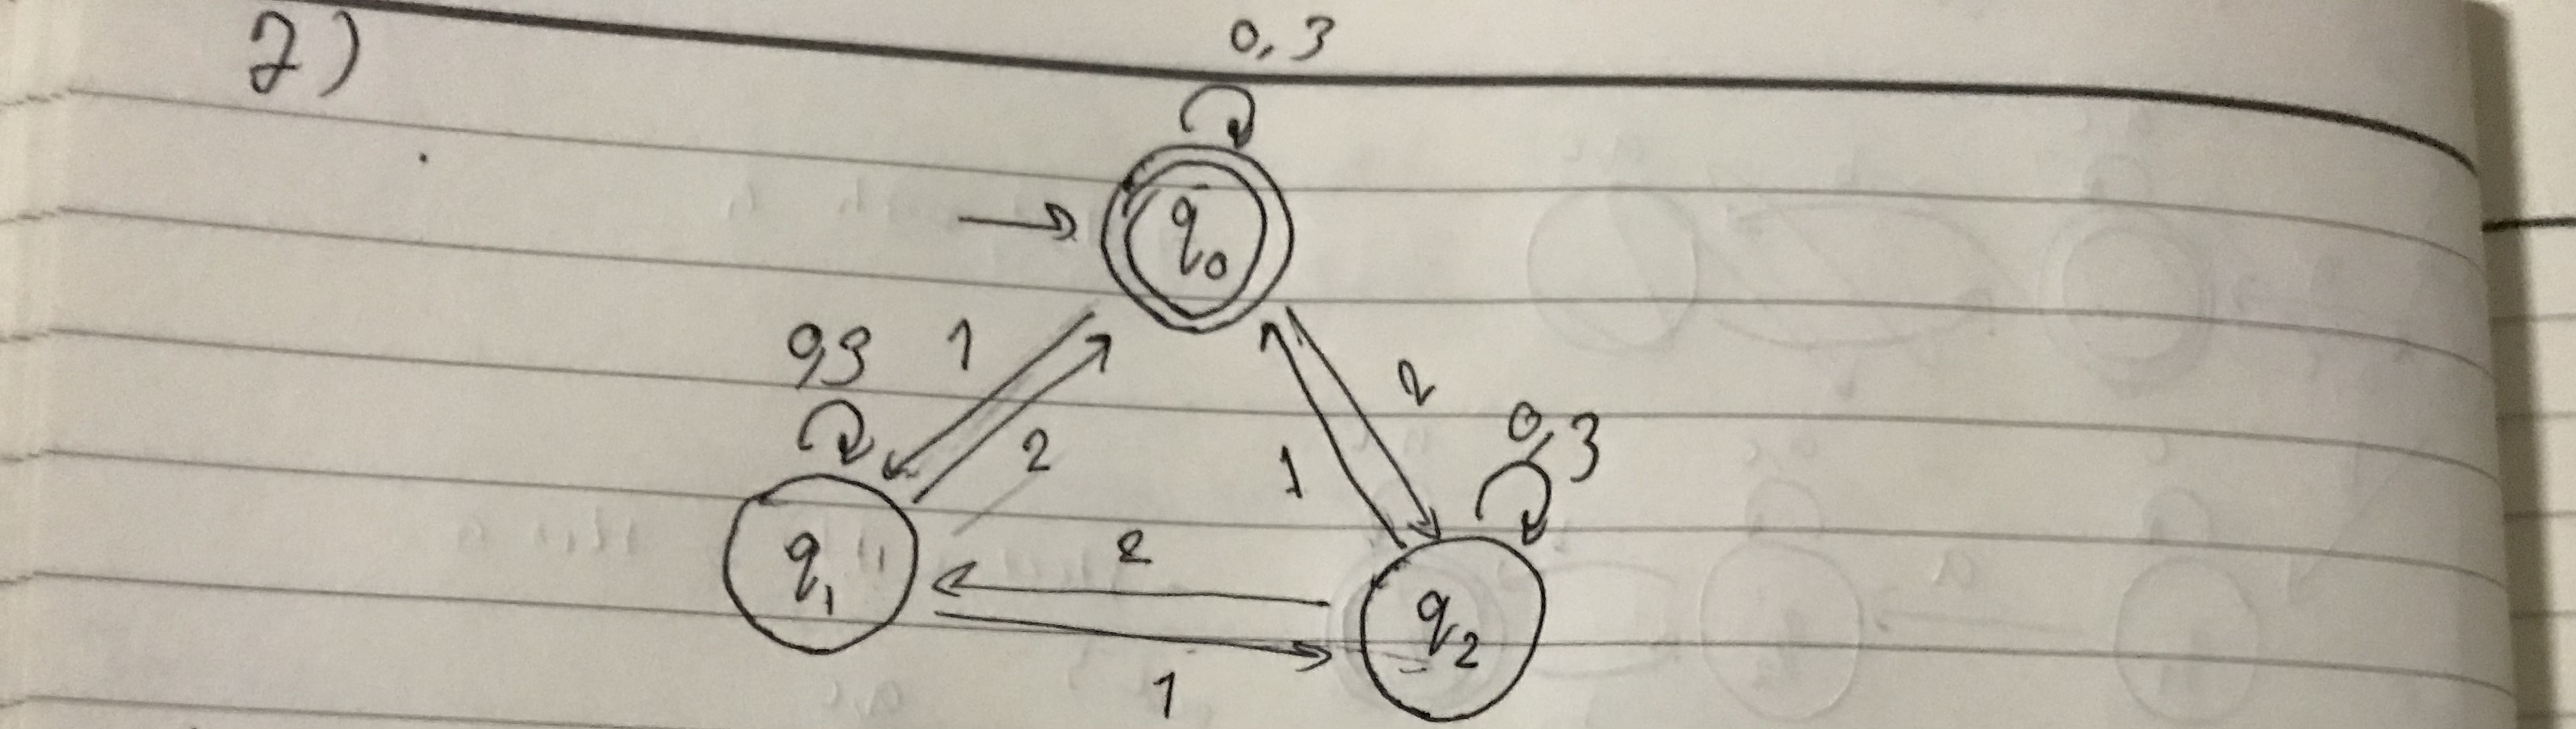
\includegraphics[width=\textwidth]{Q7_new_new.png}\\
 \begin{enumerate}
 	\item $q_0$ - accepting state. If character is 0 or 3 stay the at $q_0$ as it is alsal accepting state.
 	\item $q_0$ to $q_1$ - the character is one then you need either $1+1$ or 2.
 	\item $q_1$ to $q_0$ - we got 2 so we already have 3 so go back to $q_0$.
 	\item $q_1$ to $q_2$ to $q_3$ - $1 + 1 + 1$ so it is divisible by 3.
 	\item $q_0$ to $q_2$ - we got the sum of 2 we need either 1 or $2+2$.
 	\item $q_2$ to $q_0$ - We alreay have 1b so it is already divisible by 3. So counter is reset.
 	\item $q_2$ to $q_1$ to $q_0$ - We have $2*3$ so 6. Six is divisible by 3 so back to $q_0$.
 \end{enumerate}
 
\end{document}

